\batchmode
\documentclass[twoside]{book}

% Packages required by doxygen
\usepackage{fixltx2e}
\usepackage{calc}
\usepackage{doxygen}
\usepackage[export]{adjustbox} % also loads graphicx
\usepackage{graphicx}
\usepackage[utf8]{inputenc}
\usepackage{makeidx}
\usepackage{multicol}
\usepackage{multirow}
\PassOptionsToPackage{warn}{textcomp}
\usepackage{textcomp}
\usepackage[nointegrals]{wasysym}
\usepackage[table]{xcolor}

% Font selection
\usepackage[T1]{fontenc}
\usepackage[scaled=.90]{helvet}
\usepackage{courier}
\usepackage{amssymb}
\usepackage{sectsty}
\renewcommand{\familydefault}{\sfdefault}
\allsectionsfont{%
  \fontseries{bc}\selectfont%
  \color{darkgray}%
}
\renewcommand{\DoxyLabelFont}{%
  \fontseries{bc}\selectfont%
  \color{darkgray}%
}
\newcommand{\+}{\discretionary{\mbox{\scriptsize$\hookleftarrow$}}{}{}}

% Page & text layout
\usepackage{geometry}
\geometry{%
  a4paper,%
  top=2.5cm,%
  bottom=2.5cm,%
  left=2.5cm,%
  right=2.5cm%
}
\tolerance=750
\hfuzz=15pt
\hbadness=750
\setlength{\emergencystretch}{15pt}
\setlength{\parindent}{0cm}
\setlength{\parskip}{3ex plus 2ex minus 2ex}
\makeatletter
\renewcommand{\paragraph}{%
  \@startsection{paragraph}{4}{0ex}{-1.0ex}{1.0ex}{%
    \normalfont\normalsize\bfseries\SS@parafont%
  }%
}
\renewcommand{\subparagraph}{%
  \@startsection{subparagraph}{5}{0ex}{-1.0ex}{1.0ex}{%
    \normalfont\normalsize\bfseries\SS@subparafont%
  }%
}
\makeatother

% Headers & footers
\usepackage{fancyhdr}
\pagestyle{fancyplain}
\fancyhead[LE]{\fancyplain{}{\bfseries\thepage}}
\fancyhead[CE]{\fancyplain{}{}}
\fancyhead[RE]{\fancyplain{}{\bfseries\leftmark}}
\fancyhead[LO]{\fancyplain{}{\bfseries\rightmark}}
\fancyhead[CO]{\fancyplain{}{}}
\fancyhead[RO]{\fancyplain{}{\bfseries\thepage}}
\fancyfoot[LE]{\fancyplain{}{}}
\fancyfoot[CE]{\fancyplain{}{}}
\fancyfoot[RE]{\fancyplain{}{\bfseries\scriptsize Generated by Doxygen }}
\fancyfoot[LO]{\fancyplain{}{\bfseries\scriptsize Generated by Doxygen }}
\fancyfoot[CO]{\fancyplain{}{}}
\fancyfoot[RO]{\fancyplain{}{}}
\renewcommand{\footrulewidth}{0.4pt}
\renewcommand{\chaptermark}[1]{%
  \markboth{#1}{}%
}
\renewcommand{\sectionmark}[1]{%
  \markright{\thesection\ #1}%
}

% Indices & bibliography
\usepackage{natbib}
\usepackage[titles]{tocloft}
\setcounter{tocdepth}{3}
\setcounter{secnumdepth}{5}
\makeindex

% Hyperlinks (required, but should be loaded last)
\usepackage{ifpdf}
\ifpdf
  \usepackage[pdftex,pagebackref=true]{hyperref}
\else
  \usepackage[ps2pdf,pagebackref=true]{hyperref}
\fi
\hypersetup{%
  colorlinks=true,%
  linkcolor=blue,%
  citecolor=blue,%
  unicode%
}

% Custom commands
\newcommand{\clearemptydoublepage}{%
  \newpage{\pagestyle{empty}\cleardoublepage}%
}

\usepackage{caption}
\captionsetup{labelsep=space,justification=centering,font={bf},singlelinecheck=off,skip=4pt,position=top}

%===== C O N T E N T S =====

\begin{document}

% Titlepage & ToC
\hypersetup{pageanchor=false,
             bookmarksnumbered=true,
             pdfencoding=unicode
            }
\pagenumbering{alph}
\pagenumbering{arabic}
\hypersetup{pageanchor=true}

%--- Begin generated contents ---
\chapter{Demo problem\+: Bending of a 3D non-\/symmetric cantilever beam made of incompressible material}
\label{index}\hypertarget{index}{}\hypertarget{index_q}{}\section{A few quick questions...}\label{index_q}
Since {\ttfamily oomph-\/lib} is developed as open-\/source software, any evidence that the code is being downloaded and used is very helpful for us as it helps to justify our continued work on this project.

We would therefore be extremely grateful if you could provide the information requested in the form below. Pressing the \char`\"{}submit\char`\"{} button will get you to the actual download page.

{\bfseries Note\+:} 
\begin{DoxyItemize}
\item All information will be treated as confidential. 
\item If you provide your email address and check the appropriate box we will add you to our mailing list to inform you of upgrades and bug fixes to the code. Rest assured that the mailing list is {\bfseries very low volume} -- we have better things to do than to bombard you with email. 
\item If you still feel reluctant to provide any of the information requested, feel free to enter some dummy input. The form will check that {\bfseries some} information has been entered but entering your name as \char`\"{}\+Joe Cool\char`\"{} is perfectly acceptable -- this is to discourage people from not providing the information simply because they are too lazy to type... 
\end{DoxyItemize}



 







 

 \hypertarget{index_pdf}{}\section{P\+D\+F file}\label{index_pdf}
A \href{../latex/refman.pdf}{\tt pdf version} of this document is available. \end{document}

\chapter{Namespace Index}
\section{Namespace List}
Here is a list of all namespaces with brief descriptions\+:\begin{DoxyCompactList}
\item\contentsline{section}{\hyperlink{namespaceGlobal__Physical__Variables}{Global\+\_\+\+Physical\+\_\+\+Variables} \\*Global variables that represent physical properties }{\pageref{namespaceGlobal__Physical__Variables}}{}
\item\contentsline{section}{\hyperlink{namespaceoomph}{oomph} }{\pageref{namespaceoomph}}{}
\item\contentsline{section}{\hyperlink{namespacePhysical__Variables}{Physical\+\_\+\+Variables} \\*Namespace for the solution of 2D linear shell equation }{\pageref{namespacePhysical__Variables}}{}
\end{DoxyCompactList}

\chapter{Hierarchical Index}
\section{Class Hierarchy}
This inheritance list is sorted roughly, but not completely, alphabetically\+:\begin{DoxyCompactList}
\item Problem\begin{DoxyCompactList}
\item \contentsline{section}{Unstructured\+Solid\+Problem$<$ E\+L\+E\+M\+E\+NT $>$}{\pageref{classUnstructuredSolidProblem}}{}
\end{DoxyCompactList}
\end{DoxyCompactList}

\chapter{Class Index}
\section{Class List}
Here are the classes, structs, unions and interfaces with brief descriptions\+:\begin{DoxyCompactList}
\item\contentsline{section}{\hyperlink{classPMLProblem}{P\+M\+L\+Problem$<$ E\+L\+E\+M\+E\+N\+T $>$} }{\pageref{classPMLProblem}}{}
\item\contentsline{section}{\hyperlink{classGlobalParameters_1_1TestPMLMapping}{Global\+Parameters\+::\+Test\+P\+M\+L\+Mapping} }{\pageref{classGlobalParameters_1_1TestPMLMapping}}{}
\end{DoxyCompactList}

\chapter{File Index}
\section{File List}
Here is a list of all files with brief descriptions\+:\begin{DoxyCompactList}
\item\contentsline{section}{\hyperlink{jeffery__orbit_8cc}{jeffery\+\_\+orbit.\+cc} }{\pageref{jeffery__orbit_8cc}}{}
\item\contentsline{section}{\hyperlink{jeffery__orbit_8txt__doxygenified_8h}{jeffery\+\_\+orbit.\+txt\+\_\+doxygenified.\+h} }{\pageref{jeffery__orbit_8txt__doxygenified_8h}}{}
\item\contentsline{section}{\hyperlink{my__taylor__hood__elements_8h}{my\+\_\+taylor\+\_\+hood\+\_\+elements.\+h} }{\pageref{my__taylor__hood__elements_8h}}{}
\end{DoxyCompactList}

\chapter{Namespace Documentation}
\hypertarget{namespaceGlobal__Physical__Variables}{}\section{Global\+\_\+\+Physical\+\_\+\+Variables Namespace Reference}
\label{namespaceGlobal__Physical__Variables}\index{Global\+\_\+\+Physical\+\_\+\+Variables@{Global\+\_\+\+Physical\+\_\+\+Variables}}


Namespace for physical parameters.  


\subsection*{Functions}
\begin{DoxyCompactItemize}
\item 
Vector$<$ double $>$ \hyperlink{namespaceGlobal__Physical__Variables_afae321364975eb56688ad13abc8ed6b7}{Gravity} (2)
\begin{DoxyCompactList}\small\item\em Gravity vector. \end{DoxyCompactList}\item 
void \hyperlink{namespaceGlobal__Physical__Variables_a87da705b8a46bed337cf5dbdd788b87b}{body\+\_\+force} (const double \&time, const Vector$<$ double $>$ \&x, Vector$<$ double $>$ \&result)
\begin{DoxyCompactList}\small\item\em Functional body force. \end{DoxyCompactList}\item 
void \hyperlink{namespaceGlobal__Physical__Variables_a9780d615ae07c4e00a436ab2973b54e6}{zero\+\_\+body\+\_\+force} (const double \&time, const Vector$<$ double $>$ \&x, Vector$<$ double $>$ \&result)
\begin{DoxyCompactList}\small\item\em Zero functional body force. \end{DoxyCompactList}\end{DoxyCompactItemize}
\subsection*{Variables}
\begin{DoxyCompactItemize}
\item 
double \hyperlink{namespaceGlobal__Physical__Variables_ab814e627d2eb5bc50318879d19ab16b9}{Re} =100
\begin{DoxyCompactList}\small\item\em Reynolds number. \end{DoxyCompactList}\item 
double \hyperlink{namespaceGlobal__Physical__Variables_ab1a845a672b4d74b304639a976dc65c6}{Re\+\_\+inv\+Fr} =100
\begin{DoxyCompactList}\small\item\em Reynolds/\+Froude number. \end{DoxyCompactList}\end{DoxyCompactItemize}


\subsection{Detailed Description}
Namespace for physical parameters. 

\subsection{Function Documentation}
\mbox{\Hypertarget{namespaceGlobal__Physical__Variables_a87da705b8a46bed337cf5dbdd788b87b}\label{namespaceGlobal__Physical__Variables_a87da705b8a46bed337cf5dbdd788b87b}} 
\index{Global\+\_\+\+Physical\+\_\+\+Variables@{Global\+\_\+\+Physical\+\_\+\+Variables}!body\+\_\+force@{body\+\_\+force}}
\index{body\+\_\+force@{body\+\_\+force}!Global\+\_\+\+Physical\+\_\+\+Variables@{Global\+\_\+\+Physical\+\_\+\+Variables}}
\subsubsection{\texorpdfstring{body\+\_\+force()}{body\_force()}}
{\footnotesize\ttfamily void Global\+\_\+\+Physical\+\_\+\+Variables\+::body\+\_\+force (\begin{DoxyParamCaption}\item[{const double \&}]{time,  }\item[{const Vector$<$ double $>$ \&}]{x,  }\item[{Vector$<$ double $>$ \&}]{result }\end{DoxyParamCaption})}



Functional body force. 



Definition at line 62 of file circular\+\_\+driven\+\_\+cavity.\+cc.



References Re\+\_\+inv\+Fr.



Referenced by main().

\mbox{\Hypertarget{namespaceGlobal__Physical__Variables_afae321364975eb56688ad13abc8ed6b7}\label{namespaceGlobal__Physical__Variables_afae321364975eb56688ad13abc8ed6b7}} 
\index{Global\+\_\+\+Physical\+\_\+\+Variables@{Global\+\_\+\+Physical\+\_\+\+Variables}!Gravity@{Gravity}}
\index{Gravity@{Gravity}!Global\+\_\+\+Physical\+\_\+\+Variables@{Global\+\_\+\+Physical\+\_\+\+Variables}}
\subsubsection{\texorpdfstring{Gravity()}{Gravity()}}
{\footnotesize\ttfamily Vector$<$double$>$ Global\+\_\+\+Physical\+\_\+\+Variables\+::\+Gravity (\begin{DoxyParamCaption}\item[{2}]{ }\end{DoxyParamCaption})}



Gravity vector. 



Referenced by main(), and Quarter\+Circle\+Driven\+Cavity\+Problem$<$ E\+L\+E\+M\+E\+N\+T $>$\+::\+Quarter\+Circle\+Driven\+Cavity\+Problem().

\mbox{\Hypertarget{namespaceGlobal__Physical__Variables_a9780d615ae07c4e00a436ab2973b54e6}\label{namespaceGlobal__Physical__Variables_a9780d615ae07c4e00a436ab2973b54e6}} 
\index{Global\+\_\+\+Physical\+\_\+\+Variables@{Global\+\_\+\+Physical\+\_\+\+Variables}!zero\+\_\+body\+\_\+force@{zero\+\_\+body\+\_\+force}}
\index{zero\+\_\+body\+\_\+force@{zero\+\_\+body\+\_\+force}!Global\+\_\+\+Physical\+\_\+\+Variables@{Global\+\_\+\+Physical\+\_\+\+Variables}}
\subsubsection{\texorpdfstring{zero\+\_\+body\+\_\+force()}{zero\_body\_force()}}
{\footnotesize\ttfamily void Global\+\_\+\+Physical\+\_\+\+Variables\+::zero\+\_\+body\+\_\+force (\begin{DoxyParamCaption}\item[{const double \&}]{time,  }\item[{const Vector$<$ double $>$ \&}]{x,  }\item[{Vector$<$ double $>$ \&}]{result }\end{DoxyParamCaption})}



Zero functional body force. 



Definition at line 70 of file circular\+\_\+driven\+\_\+cavity.\+cc.



Referenced by main().



\subsection{Variable Documentation}
\mbox{\Hypertarget{namespaceGlobal__Physical__Variables_ab814e627d2eb5bc50318879d19ab16b9}\label{namespaceGlobal__Physical__Variables_ab814e627d2eb5bc50318879d19ab16b9}} 
\index{Global\+\_\+\+Physical\+\_\+\+Variables@{Global\+\_\+\+Physical\+\_\+\+Variables}!Re@{Re}}
\index{Re@{Re}!Global\+\_\+\+Physical\+\_\+\+Variables@{Global\+\_\+\+Physical\+\_\+\+Variables}}
\subsubsection{\texorpdfstring{Re}{Re}}
{\footnotesize\ttfamily double Global\+\_\+\+Physical\+\_\+\+Variables\+::\+Re =100}



Reynolds number. 



Definition at line 53 of file circular\+\_\+driven\+\_\+cavity.\+cc.



Referenced by Quarter\+Circle\+Driven\+Cavity\+Problem$<$ E\+L\+E\+M\+E\+N\+T $>$\+::\+Quarter\+Circle\+Driven\+Cavity\+Problem().

\mbox{\Hypertarget{namespaceGlobal__Physical__Variables_ab1a845a672b4d74b304639a976dc65c6}\label{namespaceGlobal__Physical__Variables_ab1a845a672b4d74b304639a976dc65c6}} 
\index{Global\+\_\+\+Physical\+\_\+\+Variables@{Global\+\_\+\+Physical\+\_\+\+Variables}!Re\+\_\+inv\+Fr@{Re\+\_\+inv\+Fr}}
\index{Re\+\_\+inv\+Fr@{Re\+\_\+inv\+Fr}!Global\+\_\+\+Physical\+\_\+\+Variables@{Global\+\_\+\+Physical\+\_\+\+Variables}}
\subsubsection{\texorpdfstring{Re\+\_\+inv\+Fr}{Re\_invFr}}
{\footnotesize\ttfamily double Global\+\_\+\+Physical\+\_\+\+Variables\+::\+Re\+\_\+inv\+Fr =100}



Reynolds/\+Froude number. 



Definition at line 56 of file circular\+\_\+driven\+\_\+cavity.\+cc.



Referenced by body\+\_\+force(), and Quarter\+Circle\+Driven\+Cavity\+Problem$<$ E\+L\+E\+M\+E\+N\+T $>$\+::\+Quarter\+Circle\+Driven\+Cavity\+Problem().


\chapter{Class Documentation}
\hypertarget{classCantileverProblem}{}\section{Cantilever\+Problem$<$ E\+L\+E\+M\+E\+NT $>$ Class Template Reference}
\label{classCantileverProblem}\index{Cantilever\+Problem$<$ E\+L\+E\+M\+E\+N\+T $>$@{Cantilever\+Problem$<$ E\+L\+E\+M\+E\+N\+T $>$}}


Problem class for the cantilever \char`\"{}beam\char`\"{} structure.  


Inheritance diagram for Cantilever\+Problem$<$ E\+L\+E\+M\+E\+NT $>$\+:\begin{figure}[H]
\begin{center}
\leavevmode
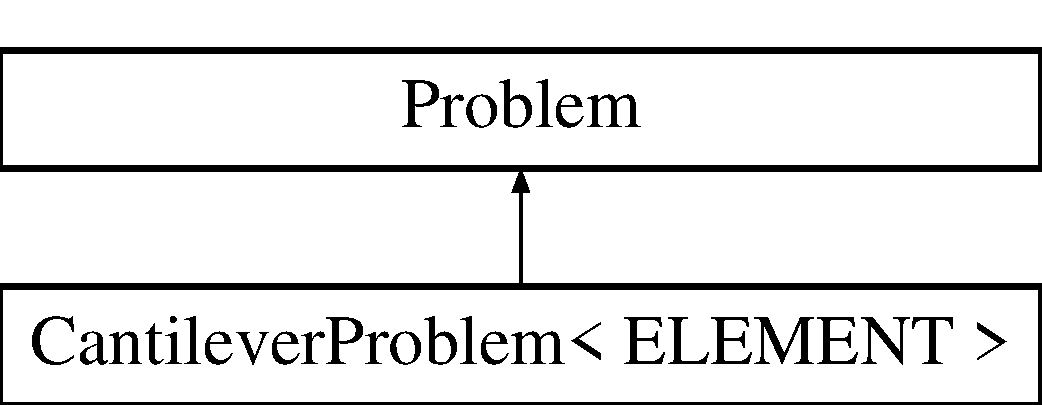
\includegraphics[height=2.000000cm]{classCantileverProblem}
\end{center}
\end{figure}
\subsection*{Public Member Functions}
\begin{DoxyCompactItemize}
\item 
\hyperlink{classCantileverProblem_abba97fc4b8402bc0363fdf16322f6572}{Cantilever\+Problem} ()
\begin{DoxyCompactList}\small\item\em Constructor\+: \end{DoxyCompactList}\item 
void \hyperlink{classCantileverProblem_a4a70a4328d287aaa15c7811562122013}{actions\+\_\+after\+\_\+newton\+\_\+solve} ()
\begin{DoxyCompactList}\small\item\em Update function (empty) \end{DoxyCompactList}\item 
void \hyperlink{classCantileverProblem_a293902b825898ce043ffce3f0691f5a5}{actions\+\_\+before\+\_\+newton\+\_\+solve} ()
\begin{DoxyCompactList}\small\item\em Update function (empty) \end{DoxyCompactList}\item 
Elastic\+Refineable\+Rectangular\+Quad\+Mesh$<$ E\+L\+E\+M\+E\+NT $>$ $\ast$\& \hyperlink{classCantileverProblem_a26843782873897ee5e45647d17204b86}{solid\+\_\+mesh\+\_\+pt} ()
\begin{DoxyCompactList}\small\item\em Access function for the solid mesh. \end{DoxyCompactList}\item 
Solid\+Mesh $\ast$\& \hyperlink{classCantileverProblem_af9e9b4a4686ac29bc7e4ef5d6baeae5a}{traction\+\_\+mesh\+\_\+pt} ()
\begin{DoxyCompactList}\small\item\em Access function to the mesh of surface traction elements. \end{DoxyCompactList}\item 
void \hyperlink{classCantileverProblem_a50f8964219c507562945655e0ed5fc23}{actions\+\_\+before\+\_\+adapt} ()
\begin{DoxyCompactList}\small\item\em Actions before adapt\+: Wipe the mesh of traction elements. \end{DoxyCompactList}\item 
void \hyperlink{classCantileverProblem_af4d135ace3eac657b38de362e1644c75}{actions\+\_\+after\+\_\+adapt} ()
\begin{DoxyCompactList}\small\item\em Actions after adapt\+: Rebuild the mesh of traction elements. \end{DoxyCompactList}\item 
void \hyperlink{classCantileverProblem_a7571348f8724e71be4e67dc64cea3877}{doc\+\_\+solution} ()
\begin{DoxyCompactList}\small\item\em Doc the solution. \end{DoxyCompactList}\item 
\hyperlink{classCantileverProblem_a83b396aa3bd0c2d9a491c605c208de83}{Cantilever\+Problem} (const bool \&incompress, const bool \&use\+\_\+fd)
\begin{DoxyCompactList}\small\item\em Constructor\+: \end{DoxyCompactList}\item 
void \hyperlink{classCantileverProblem_a4a70a4328d287aaa15c7811562122013}{actions\+\_\+after\+\_\+newton\+\_\+solve} ()
\begin{DoxyCompactList}\small\item\em Update function (empty) \end{DoxyCompactList}\item 
void \hyperlink{classCantileverProblem_a293902b825898ce043ffce3f0691f5a5}{actions\+\_\+before\+\_\+newton\+\_\+solve} ()
\begin{DoxyCompactList}\small\item\em Update function (empty) \end{DoxyCompactList}\item 
Elastic\+Refineable\+Rectangular\+Quad\+Mesh$<$ E\+L\+E\+M\+E\+NT $>$ $\ast$\& \hyperlink{classCantileverProblem_a26843782873897ee5e45647d17204b86}{solid\+\_\+mesh\+\_\+pt} ()
\begin{DoxyCompactList}\small\item\em Access function for the solid mesh. \end{DoxyCompactList}\item 
Elastic\+Rectangular\+Quad\+Mesh$<$ E\+L\+E\+M\+E\+NT $>$ $\ast$\& \hyperlink{classCantileverProblem_a63d315bcebba1a439e4b5ec0fec5b6ab}{solid\+\_\+mesh\+\_\+pt} ()
\begin{DoxyCompactList}\small\item\em Access function for the solid mesh. \end{DoxyCompactList}\item 
Solid\+Mesh $\ast$\& \hyperlink{classCantileverProblem_af9e9b4a4686ac29bc7e4ef5d6baeae5a}{traction\+\_\+mesh\+\_\+pt} ()
\begin{DoxyCompactList}\small\item\em Access function to the mesh of surface traction elements. \end{DoxyCompactList}\item 
void \hyperlink{classCantileverProblem_a50f8964219c507562945655e0ed5fc23}{actions\+\_\+before\+\_\+adapt} ()
\begin{DoxyCompactList}\small\item\em Actions before adapt\+: Wipe the mesh of traction elements. \end{DoxyCompactList}\item 
void \hyperlink{classCantileverProblem_af4d135ace3eac657b38de362e1644c75}{actions\+\_\+after\+\_\+adapt} ()
\begin{DoxyCompactList}\small\item\em Actions after adapt\+: Rebuild the mesh of traction elements. \end{DoxyCompactList}\item 
void \hyperlink{classCantileverProblem_a7571348f8724e71be4e67dc64cea3877}{doc\+\_\+solution} ()
\begin{DoxyCompactList}\small\item\em Doc the solution. \end{DoxyCompactList}\item 
void \hyperlink{classCantileverProblem_a5c78c6602e0cbeac68239804c2d52243}{run\+\_\+it} (const unsigned \&i\+\_\+case)
\begin{DoxyCompactList}\small\item\em Run the job -- doc in R\+E\+S\+L\+Ti\+\_\+case. \end{DoxyCompactList}\end{DoxyCompactItemize}
\subsection*{Private Member Functions}
\begin{DoxyCompactItemize}
\item 
void \hyperlink{classCantileverProblem_a96a9716947a15930f3881fcec6d448e2}{set\+\_\+traction\+\_\+pt} ()
\begin{DoxyCompactList}\small\item\em Pass pointer to traction function to the elements in the traction mesh. \end{DoxyCompactList}\item 
void \hyperlink{classCantileverProblem_abb6f19d964d96a531bf1a60732c72ce9}{create\+\_\+traction\+\_\+elements} ()
\begin{DoxyCompactList}\small\item\em Create traction elements. \end{DoxyCompactList}\item 
void \hyperlink{classCantileverProblem_aeb64122ce3783bf36df3696c41e5d2a5}{delete\+\_\+traction\+\_\+elements} ()
\begin{DoxyCompactList}\small\item\em Delete traction elements. \end{DoxyCompactList}\item 
void \hyperlink{classCantileverProblem_a96a9716947a15930f3881fcec6d448e2}{set\+\_\+traction\+\_\+pt} ()
\begin{DoxyCompactList}\small\item\em Pass pointer to traction function to the elements in the traction mesh. \end{DoxyCompactList}\item 
void \hyperlink{classCantileverProblem_abb6f19d964d96a531bf1a60732c72ce9}{create\+\_\+traction\+\_\+elements} ()
\begin{DoxyCompactList}\small\item\em Create traction elements. \end{DoxyCompactList}\item 
void \hyperlink{classCantileverProblem_aeb64122ce3783bf36df3696c41e5d2a5}{delete\+\_\+traction\+\_\+elements} ()
\begin{DoxyCompactList}\small\item\em Delete traction elements. \end{DoxyCompactList}\end{DoxyCompactItemize}
\subsection*{Private Attributes}
\begin{DoxyCompactItemize}
\item 
ofstream \hyperlink{classCantileverProblem_af1e298e0b99bddc89b20da6ad4bb41e1}{Trace\+\_\+file}
\begin{DoxyCompactList}\small\item\em Trace file. \end{DoxyCompactList}\item 
Node $\ast$ \hyperlink{classCantileverProblem_a7b91e041c3e5336b62ced10774917370}{Trace\+\_\+node\+\_\+pt}
\begin{DoxyCompactList}\small\item\em Pointers to node whose position we\textquotesingle{}re tracing. \end{DoxyCompactList}\item 
Elastic\+Refineable\+Rectangular\+Quad\+Mesh$<$ E\+L\+E\+M\+E\+NT $>$ $\ast$ \hyperlink{classCantileverProblem_a263ff19e4aa0fa4391582242763f08f1}{Solid\+\_\+mesh\+\_\+pt}
\begin{DoxyCompactList}\small\item\em Pointer to solid mesh. \end{DoxyCompactList}\item 
Solid\+Mesh $\ast$ \hyperlink{classCantileverProblem_a52485434aab5d653010c48a0b0f89088}{Traction\+\_\+mesh\+\_\+pt}
\begin{DoxyCompactList}\small\item\em Pointer to mesh of traction elements. \end{DoxyCompactList}\item 
Doc\+Info \hyperlink{classCantileverProblem_a2d230bb59f229cf02a06a50493dd48e4}{Doc\+\_\+info}
\begin{DoxyCompactList}\small\item\em Doc\+Info object for output. \end{DoxyCompactList}\item 
Elastic\+Rectangular\+Quad\+Mesh$<$ E\+L\+E\+M\+E\+NT $>$ $\ast$ \hyperlink{classCantileverProblem_af46dcd5eca58d44f1078e54f7779f0d5}{Solid\+\_\+mesh\+\_\+pt}
\begin{DoxyCompactList}\small\item\em Pointer to solid mesh. \end{DoxyCompactList}\end{DoxyCompactItemize}


\subsection{Detailed Description}
\subsubsection*{template$<$class E\+L\+E\+M\+E\+NT$>$\newline
class Cantilever\+Problem$<$ E\+L\+E\+M\+E\+N\+T $>$}

Problem class for the cantilever \char`\"{}beam\char`\"{} structure. 

Definition at line 209 of file airy\+\_\+cantilever.\+cc.



\subsection{Constructor \& Destructor Documentation}
\mbox{\Hypertarget{classCantileverProblem_abba97fc4b8402bc0363fdf16322f6572}\label{classCantileverProblem_abba97fc4b8402bc0363fdf16322f6572}} 
\index{Cantilever\+Problem@{Cantilever\+Problem}!Cantilever\+Problem@{Cantilever\+Problem}}
\index{Cantilever\+Problem@{Cantilever\+Problem}!Cantilever\+Problem@{Cantilever\+Problem}}
\subsubsection{\texorpdfstring{Cantilever\+Problem()}{CantileverProblem()}\hspace{0.1cm}{\footnotesize\ttfamily [1/2]}}
{\footnotesize\ttfamily template$<$class E\+L\+E\+M\+E\+NT $>$ \\
\hyperlink{classCantileverProblem}{Cantilever\+Problem}$<$ E\+L\+E\+M\+E\+NT $>$\+::\hyperlink{classCantileverProblem}{Cantilever\+Problem} (\begin{DoxyParamCaption}{ }\end{DoxyParamCaption})}



Constructor\+: 



Definition at line 273 of file airy\+\_\+cantilever.\+cc.



References Global\+\_\+\+Physical\+\_\+\+Variables\+::\+Constitutive\+\_\+law\+\_\+pt, Global\+\_\+\+Physical\+\_\+\+Variables\+::gravity(), Global\+\_\+\+Physical\+\_\+\+Variables\+::H, and Global\+\_\+\+Physical\+\_\+\+Variables\+::L.

\mbox{\Hypertarget{classCantileverProblem_a83b396aa3bd0c2d9a491c605c208de83}\label{classCantileverProblem_a83b396aa3bd0c2d9a491c605c208de83}} 
\index{Cantilever\+Problem@{Cantilever\+Problem}!Cantilever\+Problem@{Cantilever\+Problem}}
\index{Cantilever\+Problem@{Cantilever\+Problem}!Cantilever\+Problem@{Cantilever\+Problem}}
\subsubsection{\texorpdfstring{Cantilever\+Problem()}{CantileverProblem()}\hspace{0.1cm}{\footnotesize\ttfamily [2/2]}}
{\footnotesize\ttfamily template$<$class E\+L\+E\+M\+E\+NT $>$ \\
\hyperlink{classCantileverProblem}{Cantilever\+Problem}$<$ E\+L\+E\+M\+E\+NT $>$\+::\hyperlink{classCantileverProblem}{Cantilever\+Problem} (\begin{DoxyParamCaption}\item[{const bool \&}]{incompress,  }\item[{const bool \&}]{use\+\_\+fd }\end{DoxyParamCaption})}



Constructor\+: 



Definition at line 310 of file airy\+\_\+cantilever2.\+cc.



References Cantilever\+Problem$<$ E\+L\+E\+M\+E\+N\+T $>$\+::actions\+\_\+after\+\_\+adapt(), Cantilever\+Problem$<$ E\+L\+E\+M\+E\+N\+T $>$\+::actions\+\_\+before\+\_\+adapt(), Global\+\_\+\+Physical\+\_\+\+Variables\+::constant\+\_\+pressure(), Global\+\_\+\+Physical\+\_\+\+Variables\+::\+Constitutive\+\_\+law\+\_\+pt, Cantilever\+Problem$<$ E\+L\+E\+M\+E\+N\+T $>$\+::create\+\_\+traction\+\_\+elements(), Cantilever\+Problem$<$ E\+L\+E\+M\+E\+N\+T $>$\+::delete\+\_\+traction\+\_\+elements(), Cantilever\+Problem$<$ E\+L\+E\+M\+E\+N\+T $>$\+::doc\+\_\+solution(), Global\+\_\+\+Physical\+\_\+\+Variables\+::gravity(), Global\+\_\+\+Physical\+\_\+\+Variables\+::H, Global\+\_\+\+Physical\+\_\+\+Variables\+::L, Global\+\_\+\+Physical\+\_\+\+Variables\+::P, and Cantilever\+Problem$<$ E\+L\+E\+M\+E\+N\+T $>$\+::set\+\_\+traction\+\_\+pt().



\subsection{Member Function Documentation}
\mbox{\Hypertarget{classCantileverProblem_af4d135ace3eac657b38de362e1644c75}\label{classCantileverProblem_af4d135ace3eac657b38de362e1644c75}} 
\index{Cantilever\+Problem@{Cantilever\+Problem}!actions\+\_\+after\+\_\+adapt@{actions\+\_\+after\+\_\+adapt}}
\index{actions\+\_\+after\+\_\+adapt@{actions\+\_\+after\+\_\+adapt}!Cantilever\+Problem@{Cantilever\+Problem}}
\subsubsection{\texorpdfstring{actions\+\_\+after\+\_\+adapt()}{actions\_after\_adapt()}\hspace{0.1cm}{\footnotesize\ttfamily [1/2]}}
{\footnotesize\ttfamily template$<$class E\+L\+E\+M\+E\+NT $>$ \\
void \hyperlink{classCantileverProblem}{Cantilever\+Problem}$<$ E\+L\+E\+M\+E\+NT $>$\+::actions\+\_\+after\+\_\+adapt (\begin{DoxyParamCaption}{ }\end{DoxyParamCaption})}



Actions after adapt\+: Rebuild the mesh of traction elements. 



Definition at line 392 of file airy\+\_\+cantilever.\+cc.



Referenced by Cantilever\+Problem$<$ E\+L\+E\+M\+E\+N\+T $>$\+::\+Cantilever\+Problem().

\mbox{\Hypertarget{classCantileverProblem_af4d135ace3eac657b38de362e1644c75}\label{classCantileverProblem_af4d135ace3eac657b38de362e1644c75}} 
\index{Cantilever\+Problem@{Cantilever\+Problem}!actions\+\_\+after\+\_\+adapt@{actions\+\_\+after\+\_\+adapt}}
\index{actions\+\_\+after\+\_\+adapt@{actions\+\_\+after\+\_\+adapt}!Cantilever\+Problem@{Cantilever\+Problem}}
\subsubsection{\texorpdfstring{actions\+\_\+after\+\_\+adapt()}{actions\_after\_adapt()}\hspace{0.1cm}{\footnotesize\ttfamily [2/2]}}
{\footnotesize\ttfamily template$<$class E\+L\+E\+M\+E\+NT$>$ \\
void \hyperlink{classCantileverProblem}{Cantilever\+Problem}$<$ E\+L\+E\+M\+E\+NT $>$\+::actions\+\_\+after\+\_\+adapt (\begin{DoxyParamCaption}{ }\end{DoxyParamCaption})}



Actions after adapt\+: Rebuild the mesh of traction elements. 

\mbox{\Hypertarget{classCantileverProblem_a4a70a4328d287aaa15c7811562122013}\label{classCantileverProblem_a4a70a4328d287aaa15c7811562122013}} 
\index{Cantilever\+Problem@{Cantilever\+Problem}!actions\+\_\+after\+\_\+newton\+\_\+solve@{actions\+\_\+after\+\_\+newton\+\_\+solve}}
\index{actions\+\_\+after\+\_\+newton\+\_\+solve@{actions\+\_\+after\+\_\+newton\+\_\+solve}!Cantilever\+Problem@{Cantilever\+Problem}}
\subsubsection{\texorpdfstring{actions\+\_\+after\+\_\+newton\+\_\+solve()}{actions\_after\_newton\_solve()}\hspace{0.1cm}{\footnotesize\ttfamily [1/2]}}
{\footnotesize\ttfamily template$<$class E\+L\+E\+M\+E\+NT$>$ \\
void \hyperlink{classCantileverProblem}{Cantilever\+Problem}$<$ E\+L\+E\+M\+E\+NT $>$\+::actions\+\_\+after\+\_\+newton\+\_\+solve (\begin{DoxyParamCaption}{ }\end{DoxyParamCaption})\hspace{0.3cm}{\ttfamily [inline]}}



Update function (empty) 



Definition at line 218 of file airy\+\_\+cantilever.\+cc.

\mbox{\Hypertarget{classCantileverProblem_a4a70a4328d287aaa15c7811562122013}\label{classCantileverProblem_a4a70a4328d287aaa15c7811562122013}} 
\index{Cantilever\+Problem@{Cantilever\+Problem}!actions\+\_\+after\+\_\+newton\+\_\+solve@{actions\+\_\+after\+\_\+newton\+\_\+solve}}
\index{actions\+\_\+after\+\_\+newton\+\_\+solve@{actions\+\_\+after\+\_\+newton\+\_\+solve}!Cantilever\+Problem@{Cantilever\+Problem}}
\subsubsection{\texorpdfstring{actions\+\_\+after\+\_\+newton\+\_\+solve()}{actions\_after\_newton\_solve()}\hspace{0.1cm}{\footnotesize\ttfamily [2/2]}}
{\footnotesize\ttfamily template$<$class E\+L\+E\+M\+E\+NT$>$ \\
void \hyperlink{classCantileverProblem}{Cantilever\+Problem}$<$ E\+L\+E\+M\+E\+NT $>$\+::actions\+\_\+after\+\_\+newton\+\_\+solve (\begin{DoxyParamCaption}{ }\end{DoxyParamCaption})\hspace{0.3cm}{\ttfamily [inline]}}



Update function (empty) 



Definition at line 230 of file airy\+\_\+cantilever2.\+cc.

\mbox{\Hypertarget{classCantileverProblem_a50f8964219c507562945655e0ed5fc23}\label{classCantileverProblem_a50f8964219c507562945655e0ed5fc23}} 
\index{Cantilever\+Problem@{Cantilever\+Problem}!actions\+\_\+before\+\_\+adapt@{actions\+\_\+before\+\_\+adapt}}
\index{actions\+\_\+before\+\_\+adapt@{actions\+\_\+before\+\_\+adapt}!Cantilever\+Problem@{Cantilever\+Problem}}
\subsubsection{\texorpdfstring{actions\+\_\+before\+\_\+adapt()}{actions\_before\_adapt()}\hspace{0.1cm}{\footnotesize\ttfamily [1/2]}}
{\footnotesize\ttfamily template$<$class E\+L\+E\+M\+E\+NT $>$ \\
void \hyperlink{classCantileverProblem}{Cantilever\+Problem}$<$ E\+L\+E\+M\+E\+NT $>$\+::actions\+\_\+before\+\_\+adapt (\begin{DoxyParamCaption}{ }\end{DoxyParamCaption})}



Actions before adapt\+: Wipe the mesh of traction elements. 



Definition at line 376 of file airy\+\_\+cantilever.\+cc.



Referenced by Cantilever\+Problem$<$ E\+L\+E\+M\+E\+N\+T $>$\+::\+Cantilever\+Problem().

\mbox{\Hypertarget{classCantileverProblem_a50f8964219c507562945655e0ed5fc23}\label{classCantileverProblem_a50f8964219c507562945655e0ed5fc23}} 
\index{Cantilever\+Problem@{Cantilever\+Problem}!actions\+\_\+before\+\_\+adapt@{actions\+\_\+before\+\_\+adapt}}
\index{actions\+\_\+before\+\_\+adapt@{actions\+\_\+before\+\_\+adapt}!Cantilever\+Problem@{Cantilever\+Problem}}
\subsubsection{\texorpdfstring{actions\+\_\+before\+\_\+adapt()}{actions\_before\_adapt()}\hspace{0.1cm}{\footnotesize\ttfamily [2/2]}}
{\footnotesize\ttfamily template$<$class E\+L\+E\+M\+E\+NT$>$ \\
void \hyperlink{classCantileverProblem}{Cantilever\+Problem}$<$ E\+L\+E\+M\+E\+NT $>$\+::actions\+\_\+before\+\_\+adapt (\begin{DoxyParamCaption}{ }\end{DoxyParamCaption})}



Actions before adapt\+: Wipe the mesh of traction elements. 

\mbox{\Hypertarget{classCantileverProblem_a293902b825898ce043ffce3f0691f5a5}\label{classCantileverProblem_a293902b825898ce043ffce3f0691f5a5}} 
\index{Cantilever\+Problem@{Cantilever\+Problem}!actions\+\_\+before\+\_\+newton\+\_\+solve@{actions\+\_\+before\+\_\+newton\+\_\+solve}}
\index{actions\+\_\+before\+\_\+newton\+\_\+solve@{actions\+\_\+before\+\_\+newton\+\_\+solve}!Cantilever\+Problem@{Cantilever\+Problem}}
\subsubsection{\texorpdfstring{actions\+\_\+before\+\_\+newton\+\_\+solve()}{actions\_before\_newton\_solve()}\hspace{0.1cm}{\footnotesize\ttfamily [1/2]}}
{\footnotesize\ttfamily template$<$class E\+L\+E\+M\+E\+NT$>$ \\
void \hyperlink{classCantileverProblem}{Cantilever\+Problem}$<$ E\+L\+E\+M\+E\+NT $>$\+::actions\+\_\+before\+\_\+newton\+\_\+solve (\begin{DoxyParamCaption}{ }\end{DoxyParamCaption})\hspace{0.3cm}{\ttfamily [inline]}}



Update function (empty) 



Definition at line 221 of file airy\+\_\+cantilever.\+cc.

\mbox{\Hypertarget{classCantileverProblem_a293902b825898ce043ffce3f0691f5a5}\label{classCantileverProblem_a293902b825898ce043ffce3f0691f5a5}} 
\index{Cantilever\+Problem@{Cantilever\+Problem}!actions\+\_\+before\+\_\+newton\+\_\+solve@{actions\+\_\+before\+\_\+newton\+\_\+solve}}
\index{actions\+\_\+before\+\_\+newton\+\_\+solve@{actions\+\_\+before\+\_\+newton\+\_\+solve}!Cantilever\+Problem@{Cantilever\+Problem}}
\subsubsection{\texorpdfstring{actions\+\_\+before\+\_\+newton\+\_\+solve()}{actions\_before\_newton\_solve()}\hspace{0.1cm}{\footnotesize\ttfamily [2/2]}}
{\footnotesize\ttfamily template$<$class E\+L\+E\+M\+E\+NT$>$ \\
void \hyperlink{classCantileverProblem}{Cantilever\+Problem}$<$ E\+L\+E\+M\+E\+NT $>$\+::actions\+\_\+before\+\_\+newton\+\_\+solve (\begin{DoxyParamCaption}{ }\end{DoxyParamCaption})\hspace{0.3cm}{\ttfamily [inline]}}



Update function (empty) 



Definition at line 233 of file airy\+\_\+cantilever2.\+cc.

\mbox{\Hypertarget{classCantileverProblem_abb6f19d964d96a531bf1a60732c72ce9}\label{classCantileverProblem_abb6f19d964d96a531bf1a60732c72ce9}} 
\index{Cantilever\+Problem@{Cantilever\+Problem}!create\+\_\+traction\+\_\+elements@{create\+\_\+traction\+\_\+elements}}
\index{create\+\_\+traction\+\_\+elements@{create\+\_\+traction\+\_\+elements}!Cantilever\+Problem@{Cantilever\+Problem}}
\subsubsection{\texorpdfstring{create\+\_\+traction\+\_\+elements()}{create\_traction\_elements()}\hspace{0.1cm}{\footnotesize\ttfamily [1/2]}}
{\footnotesize\ttfamily template$<$class E\+L\+E\+M\+E\+NT $>$ \\
void \hyperlink{classCantileverProblem}{Cantilever\+Problem}$<$ E\+L\+E\+M\+E\+NT $>$\+::create\+\_\+traction\+\_\+elements (\begin{DoxyParamCaption}{ }\end{DoxyParamCaption})\hspace{0.3cm}{\ttfamily [private]}}



Create traction elements. 



Definition at line 441 of file airy\+\_\+cantilever.\+cc.



Referenced by Cantilever\+Problem$<$ E\+L\+E\+M\+E\+N\+T $>$\+::\+Cantilever\+Problem().

\mbox{\Hypertarget{classCantileverProblem_abb6f19d964d96a531bf1a60732c72ce9}\label{classCantileverProblem_abb6f19d964d96a531bf1a60732c72ce9}} 
\index{Cantilever\+Problem@{Cantilever\+Problem}!create\+\_\+traction\+\_\+elements@{create\+\_\+traction\+\_\+elements}}
\index{create\+\_\+traction\+\_\+elements@{create\+\_\+traction\+\_\+elements}!Cantilever\+Problem@{Cantilever\+Problem}}
\subsubsection{\texorpdfstring{create\+\_\+traction\+\_\+elements()}{create\_traction\_elements()}\hspace{0.1cm}{\footnotesize\ttfamily [2/2]}}
{\footnotesize\ttfamily template$<$class E\+L\+E\+M\+E\+NT$>$ \\
void \hyperlink{classCantileverProblem}{Cantilever\+Problem}$<$ E\+L\+E\+M\+E\+NT $>$\+::create\+\_\+traction\+\_\+elements (\begin{DoxyParamCaption}{ }\end{DoxyParamCaption})\hspace{0.3cm}{\ttfamily [private]}}



Create traction elements. 

\mbox{\Hypertarget{classCantileverProblem_aeb64122ce3783bf36df3696c41e5d2a5}\label{classCantileverProblem_aeb64122ce3783bf36df3696c41e5d2a5}} 
\index{Cantilever\+Problem@{Cantilever\+Problem}!delete\+\_\+traction\+\_\+elements@{delete\+\_\+traction\+\_\+elements}}
\index{delete\+\_\+traction\+\_\+elements@{delete\+\_\+traction\+\_\+elements}!Cantilever\+Problem@{Cantilever\+Problem}}
\subsubsection{\texorpdfstring{delete\+\_\+traction\+\_\+elements()}{delete\_traction\_elements()}\hspace{0.1cm}{\footnotesize\ttfamily [1/2]}}
{\footnotesize\ttfamily template$<$class E\+L\+E\+M\+E\+NT $>$ \\
void \hyperlink{classCantileverProblem}{Cantilever\+Problem}$<$ E\+L\+E\+M\+E\+NT $>$\+::delete\+\_\+traction\+\_\+elements (\begin{DoxyParamCaption}{ }\end{DoxyParamCaption})\hspace{0.3cm}{\ttfamily [private]}}



Delete traction elements. 

Delete traction elements and wipe the traction meshes. 

Definition at line 476 of file airy\+\_\+cantilever.\+cc.



Referenced by Cantilever\+Problem$<$ E\+L\+E\+M\+E\+N\+T $>$\+::\+Cantilever\+Problem().

\mbox{\Hypertarget{classCantileverProblem_aeb64122ce3783bf36df3696c41e5d2a5}\label{classCantileverProblem_aeb64122ce3783bf36df3696c41e5d2a5}} 
\index{Cantilever\+Problem@{Cantilever\+Problem}!delete\+\_\+traction\+\_\+elements@{delete\+\_\+traction\+\_\+elements}}
\index{delete\+\_\+traction\+\_\+elements@{delete\+\_\+traction\+\_\+elements}!Cantilever\+Problem@{Cantilever\+Problem}}
\subsubsection{\texorpdfstring{delete\+\_\+traction\+\_\+elements()}{delete\_traction\_elements()}\hspace{0.1cm}{\footnotesize\ttfamily [2/2]}}
{\footnotesize\ttfamily template$<$class E\+L\+E\+M\+E\+NT$>$ \\
void \hyperlink{classCantileverProblem}{Cantilever\+Problem}$<$ E\+L\+E\+M\+E\+NT $>$\+::delete\+\_\+traction\+\_\+elements (\begin{DoxyParamCaption}{ }\end{DoxyParamCaption})\hspace{0.3cm}{\ttfamily [private]}}



Delete traction elements. 

\mbox{\Hypertarget{classCantileverProblem_a7571348f8724e71be4e67dc64cea3877}\label{classCantileverProblem_a7571348f8724e71be4e67dc64cea3877}} 
\index{Cantilever\+Problem@{Cantilever\+Problem}!doc\+\_\+solution@{doc\+\_\+solution}}
\index{doc\+\_\+solution@{doc\+\_\+solution}!Cantilever\+Problem@{Cantilever\+Problem}}
\subsubsection{\texorpdfstring{doc\+\_\+solution()}{doc\_solution()}\hspace{0.1cm}{\footnotesize\ttfamily [1/2]}}
{\footnotesize\ttfamily template$<$class E\+L\+E\+M\+E\+NT $>$ \\
void \hyperlink{classCantileverProblem}{Cantilever\+Problem}$<$ E\+L\+E\+M\+E\+NT $>$\+::doc\+\_\+solution (\begin{DoxyParamCaption}{ }\end{DoxyParamCaption})}



Doc the solution. 



Definition at line 499 of file airy\+\_\+cantilever.\+cc.



References Global\+\_\+\+Physical\+\_\+\+Variables\+::H, Global\+\_\+\+Physical\+\_\+\+Variables\+::L, and Global\+\_\+\+Physical\+\_\+\+Variables\+::P.



Referenced by Cantilever\+Problem$<$ E\+L\+E\+M\+E\+N\+T $>$\+::\+Cantilever\+Problem(), and main().

\mbox{\Hypertarget{classCantileverProblem_a7571348f8724e71be4e67dc64cea3877}\label{classCantileverProblem_a7571348f8724e71be4e67dc64cea3877}} 
\index{Cantilever\+Problem@{Cantilever\+Problem}!doc\+\_\+solution@{doc\+\_\+solution}}
\index{doc\+\_\+solution@{doc\+\_\+solution}!Cantilever\+Problem@{Cantilever\+Problem}}
\subsubsection{\texorpdfstring{doc\+\_\+solution()}{doc\_solution()}\hspace{0.1cm}{\footnotesize\ttfamily [2/2]}}
{\footnotesize\ttfamily template$<$class E\+L\+E\+M\+E\+NT$>$ \\
void \hyperlink{classCantileverProblem}{Cantilever\+Problem}$<$ E\+L\+E\+M\+E\+NT $>$\+::doc\+\_\+solution (\begin{DoxyParamCaption}{ }\end{DoxyParamCaption})}



Doc the solution. 

\mbox{\Hypertarget{classCantileverProblem_a5c78c6602e0cbeac68239804c2d52243}\label{classCantileverProblem_a5c78c6602e0cbeac68239804c2d52243}} 
\index{Cantilever\+Problem@{Cantilever\+Problem}!run\+\_\+it@{run\+\_\+it}}
\index{run\+\_\+it@{run\+\_\+it}!Cantilever\+Problem@{Cantilever\+Problem}}
\subsubsection{\texorpdfstring{run\+\_\+it()}{run\_it()}}
{\footnotesize\ttfamily template$<$class E\+L\+E\+M\+E\+NT $>$ \\
void \hyperlink{classCantileverProblem}{Cantilever\+Problem}$<$ E\+L\+E\+M\+E\+NT $>$\+::run\+\_\+it (\begin{DoxyParamCaption}\item[{const unsigned \&}]{i\+\_\+case }\end{DoxyParamCaption})}



Run the job -- doc in R\+E\+S\+L\+Ti\+\_\+case. 

Run it. 

Definition at line 676 of file airy\+\_\+cantilever2.\+cc.



References Global\+\_\+\+Physical\+\_\+\+Variables\+::\+Gravity, and Global\+\_\+\+Physical\+\_\+\+Variables\+::P.



Referenced by main().

\mbox{\Hypertarget{classCantileverProblem_a96a9716947a15930f3881fcec6d448e2}\label{classCantileverProblem_a96a9716947a15930f3881fcec6d448e2}} 
\index{Cantilever\+Problem@{Cantilever\+Problem}!set\+\_\+traction\+\_\+pt@{set\+\_\+traction\+\_\+pt}}
\index{set\+\_\+traction\+\_\+pt@{set\+\_\+traction\+\_\+pt}!Cantilever\+Problem@{Cantilever\+Problem}}
\subsubsection{\texorpdfstring{set\+\_\+traction\+\_\+pt()}{set\_traction\_pt()}\hspace{0.1cm}{\footnotesize\ttfamily [1/2]}}
{\footnotesize\ttfamily template$<$class E\+L\+E\+M\+E\+NT $>$ \\
void \hyperlink{classCantileverProblem}{Cantilever\+Problem}$<$ E\+L\+E\+M\+E\+NT $>$\+::set\+\_\+traction\+\_\+pt (\begin{DoxyParamCaption}{ }\end{DoxyParamCaption})\hspace{0.3cm}{\ttfamily [private]}}



Pass pointer to traction function to the elements in the traction mesh. 

Set pointer to traction function for the relevant elements in the traction mesh 

Definition at line 417 of file airy\+\_\+cantilever.\+cc.



References Global\+\_\+\+Physical\+\_\+\+Variables\+::constant\+\_\+pressure().



Referenced by Cantilever\+Problem$<$ E\+L\+E\+M\+E\+N\+T $>$\+::\+Cantilever\+Problem().

\mbox{\Hypertarget{classCantileverProblem_a96a9716947a15930f3881fcec6d448e2}\label{classCantileverProblem_a96a9716947a15930f3881fcec6d448e2}} 
\index{Cantilever\+Problem@{Cantilever\+Problem}!set\+\_\+traction\+\_\+pt@{set\+\_\+traction\+\_\+pt}}
\index{set\+\_\+traction\+\_\+pt@{set\+\_\+traction\+\_\+pt}!Cantilever\+Problem@{Cantilever\+Problem}}
\subsubsection{\texorpdfstring{set\+\_\+traction\+\_\+pt()}{set\_traction\_pt()}\hspace{0.1cm}{\footnotesize\ttfamily [2/2]}}
{\footnotesize\ttfamily template$<$class E\+L\+E\+M\+E\+NT$>$ \\
void \hyperlink{classCantileverProblem}{Cantilever\+Problem}$<$ E\+L\+E\+M\+E\+NT $>$\+::set\+\_\+traction\+\_\+pt (\begin{DoxyParamCaption}{ }\end{DoxyParamCaption})\hspace{0.3cm}{\ttfamily [private]}}



Pass pointer to traction function to the elements in the traction mesh. 

\mbox{\Hypertarget{classCantileverProblem_a26843782873897ee5e45647d17204b86}\label{classCantileverProblem_a26843782873897ee5e45647d17204b86}} 
\index{Cantilever\+Problem@{Cantilever\+Problem}!solid\+\_\+mesh\+\_\+pt@{solid\+\_\+mesh\+\_\+pt}}
\index{solid\+\_\+mesh\+\_\+pt@{solid\+\_\+mesh\+\_\+pt}!Cantilever\+Problem@{Cantilever\+Problem}}
\subsubsection{\texorpdfstring{solid\+\_\+mesh\+\_\+pt()}{solid\_mesh\_pt()}\hspace{0.1cm}{\footnotesize\ttfamily [1/3]}}
{\footnotesize\ttfamily template$<$class E\+L\+E\+M\+E\+NT$>$ \\
Elastic\+Refineable\+Rectangular\+Quad\+Mesh$<$E\+L\+E\+M\+E\+NT$>$$\ast$\& \hyperlink{classCantileverProblem}{Cantilever\+Problem}$<$ E\+L\+E\+M\+E\+NT $>$\+::solid\+\_\+mesh\+\_\+pt (\begin{DoxyParamCaption}{ }\end{DoxyParamCaption})\hspace{0.3cm}{\ttfamily [inline]}}



Access function for the solid mesh. 



Definition at line 224 of file airy\+\_\+cantilever.\+cc.

\mbox{\Hypertarget{classCantileverProblem_a26843782873897ee5e45647d17204b86}\label{classCantileverProblem_a26843782873897ee5e45647d17204b86}} 
\index{Cantilever\+Problem@{Cantilever\+Problem}!solid\+\_\+mesh\+\_\+pt@{solid\+\_\+mesh\+\_\+pt}}
\index{solid\+\_\+mesh\+\_\+pt@{solid\+\_\+mesh\+\_\+pt}!Cantilever\+Problem@{Cantilever\+Problem}}
\subsubsection{\texorpdfstring{solid\+\_\+mesh\+\_\+pt()}{solid\_mesh\_pt()}\hspace{0.1cm}{\footnotesize\ttfamily [2/3]}}
{\footnotesize\ttfamily template$<$class E\+L\+E\+M\+E\+NT$>$ \\
Elastic\+Refineable\+Rectangular\+Quad\+Mesh$<$E\+L\+E\+M\+E\+NT$>$$\ast$\& \hyperlink{classCantileverProblem}{Cantilever\+Problem}$<$ E\+L\+E\+M\+E\+NT $>$\+::solid\+\_\+mesh\+\_\+pt (\begin{DoxyParamCaption}{ }\end{DoxyParamCaption})\hspace{0.3cm}{\ttfamily [inline]}}



Access function for the solid mesh. 



Definition at line 238 of file airy\+\_\+cantilever2.\+cc.

\mbox{\Hypertarget{classCantileverProblem_a63d315bcebba1a439e4b5ec0fec5b6ab}\label{classCantileverProblem_a63d315bcebba1a439e4b5ec0fec5b6ab}} 
\index{Cantilever\+Problem@{Cantilever\+Problem}!solid\+\_\+mesh\+\_\+pt@{solid\+\_\+mesh\+\_\+pt}}
\index{solid\+\_\+mesh\+\_\+pt@{solid\+\_\+mesh\+\_\+pt}!Cantilever\+Problem@{Cantilever\+Problem}}
\subsubsection{\texorpdfstring{solid\+\_\+mesh\+\_\+pt()}{solid\_mesh\_pt()}\hspace{0.1cm}{\footnotesize\ttfamily [3/3]}}
{\footnotesize\ttfamily template$<$class E\+L\+E\+M\+E\+NT$>$ \\
Elastic\+Rectangular\+Quad\+Mesh$<$E\+L\+E\+M\+E\+NT$>$$\ast$\& \hyperlink{classCantileverProblem}{Cantilever\+Problem}$<$ E\+L\+E\+M\+E\+NT $>$\+::solid\+\_\+mesh\+\_\+pt (\begin{DoxyParamCaption}{ }\end{DoxyParamCaption})\hspace{0.3cm}{\ttfamily [inline]}}



Access function for the solid mesh. 



Definition at line 244 of file airy\+\_\+cantilever2.\+cc.

\mbox{\Hypertarget{classCantileverProblem_af9e9b4a4686ac29bc7e4ef5d6baeae5a}\label{classCantileverProblem_af9e9b4a4686ac29bc7e4ef5d6baeae5a}} 
\index{Cantilever\+Problem@{Cantilever\+Problem}!traction\+\_\+mesh\+\_\+pt@{traction\+\_\+mesh\+\_\+pt}}
\index{traction\+\_\+mesh\+\_\+pt@{traction\+\_\+mesh\+\_\+pt}!Cantilever\+Problem@{Cantilever\+Problem}}
\subsubsection{\texorpdfstring{traction\+\_\+mesh\+\_\+pt()}{traction\_mesh\_pt()}\hspace{0.1cm}{\footnotesize\ttfamily [1/2]}}
{\footnotesize\ttfamily template$<$class E\+L\+E\+M\+E\+NT$>$ \\
Solid\+Mesh$\ast$\& \hyperlink{classCantileverProblem}{Cantilever\+Problem}$<$ E\+L\+E\+M\+E\+NT $>$\+::traction\+\_\+mesh\+\_\+pt (\begin{DoxyParamCaption}{ }\end{DoxyParamCaption})\hspace{0.3cm}{\ttfamily [inline]}}



Access function to the mesh of surface traction elements. 



Definition at line 228 of file airy\+\_\+cantilever.\+cc.

\mbox{\Hypertarget{classCantileverProblem_af9e9b4a4686ac29bc7e4ef5d6baeae5a}\label{classCantileverProblem_af9e9b4a4686ac29bc7e4ef5d6baeae5a}} 
\index{Cantilever\+Problem@{Cantilever\+Problem}!traction\+\_\+mesh\+\_\+pt@{traction\+\_\+mesh\+\_\+pt}}
\index{traction\+\_\+mesh\+\_\+pt@{traction\+\_\+mesh\+\_\+pt}!Cantilever\+Problem@{Cantilever\+Problem}}
\subsubsection{\texorpdfstring{traction\+\_\+mesh\+\_\+pt()}{traction\_mesh\_pt()}\hspace{0.1cm}{\footnotesize\ttfamily [2/2]}}
{\footnotesize\ttfamily template$<$class E\+L\+E\+M\+E\+NT$>$ \\
Solid\+Mesh$\ast$\& \hyperlink{classCantileverProblem}{Cantilever\+Problem}$<$ E\+L\+E\+M\+E\+NT $>$\+::traction\+\_\+mesh\+\_\+pt (\begin{DoxyParamCaption}{ }\end{DoxyParamCaption})\hspace{0.3cm}{\ttfamily [inline]}}



Access function to the mesh of surface traction elements. 



Definition at line 251 of file airy\+\_\+cantilever2.\+cc.



\subsection{Member Data Documentation}
\mbox{\Hypertarget{classCantileverProblem_a2d230bb59f229cf02a06a50493dd48e4}\label{classCantileverProblem_a2d230bb59f229cf02a06a50493dd48e4}} 
\index{Cantilever\+Problem@{Cantilever\+Problem}!Doc\+\_\+info@{Doc\+\_\+info}}
\index{Doc\+\_\+info@{Doc\+\_\+info}!Cantilever\+Problem@{Cantilever\+Problem}}
\subsubsection{\texorpdfstring{Doc\+\_\+info}{Doc\_info}}
{\footnotesize\ttfamily template$<$class E\+L\+E\+M\+E\+NT$>$ \\
Doc\+Info \hyperlink{classCantileverProblem}{Cantilever\+Problem}$<$ E\+L\+E\+M\+E\+NT $>$\+::Doc\+\_\+info\hspace{0.3cm}{\ttfamily [private]}}



Doc\+Info object for output. 



Definition at line 264 of file airy\+\_\+cantilever.\+cc.

\mbox{\Hypertarget{classCantileverProblem_a263ff19e4aa0fa4391582242763f08f1}\label{classCantileverProblem_a263ff19e4aa0fa4391582242763f08f1}} 
\index{Cantilever\+Problem@{Cantilever\+Problem}!Solid\+\_\+mesh\+\_\+pt@{Solid\+\_\+mesh\+\_\+pt}}
\index{Solid\+\_\+mesh\+\_\+pt@{Solid\+\_\+mesh\+\_\+pt}!Cantilever\+Problem@{Cantilever\+Problem}}
\subsubsection{\texorpdfstring{Solid\+\_\+mesh\+\_\+pt}{Solid\_mesh\_pt}\hspace{0.1cm}{\footnotesize\ttfamily [1/2]}}
{\footnotesize\ttfamily template$<$class E\+L\+E\+M\+E\+NT$>$ \\
Elastic\+Refineable\+Rectangular\+Quad\+Mesh$<$ E\+L\+E\+M\+E\+NT $>$ $\ast$ \hyperlink{classCantileverProblem}{Cantilever\+Problem}$<$ E\+L\+E\+M\+E\+NT $>$\+::Solid\+\_\+mesh\+\_\+pt\hspace{0.3cm}{\ttfamily [private]}}



Pointer to solid mesh. 



Definition at line 258 of file airy\+\_\+cantilever.\+cc.

\mbox{\Hypertarget{classCantileverProblem_af46dcd5eca58d44f1078e54f7779f0d5}\label{classCantileverProblem_af46dcd5eca58d44f1078e54f7779f0d5}} 
\index{Cantilever\+Problem@{Cantilever\+Problem}!Solid\+\_\+mesh\+\_\+pt@{Solid\+\_\+mesh\+\_\+pt}}
\index{Solid\+\_\+mesh\+\_\+pt@{Solid\+\_\+mesh\+\_\+pt}!Cantilever\+Problem@{Cantilever\+Problem}}
\subsubsection{\texorpdfstring{Solid\+\_\+mesh\+\_\+pt}{Solid\_mesh\_pt}\hspace{0.1cm}{\footnotesize\ttfamily [2/2]}}
{\footnotesize\ttfamily template$<$class E\+L\+E\+M\+E\+NT$>$ \\
Elastic\+Rectangular\+Quad\+Mesh$<$E\+L\+E\+M\+E\+NT$>$$\ast$ \hyperlink{classCantileverProblem}{Cantilever\+Problem}$<$ E\+L\+E\+M\+E\+NT $>$\+::Solid\+\_\+mesh\+\_\+pt\hspace{0.3cm}{\ttfamily [private]}}



Pointer to solid mesh. 



Definition at line 292 of file airy\+\_\+cantilever2.\+cc.

\mbox{\Hypertarget{classCantileverProblem_af1e298e0b99bddc89b20da6ad4bb41e1}\label{classCantileverProblem_af1e298e0b99bddc89b20da6ad4bb41e1}} 
\index{Cantilever\+Problem@{Cantilever\+Problem}!Trace\+\_\+file@{Trace\+\_\+file}}
\index{Trace\+\_\+file@{Trace\+\_\+file}!Cantilever\+Problem@{Cantilever\+Problem}}
\subsubsection{\texorpdfstring{Trace\+\_\+file}{Trace\_file}}
{\footnotesize\ttfamily template$<$class E\+L\+E\+M\+E\+NT$>$ \\
ofstream \hyperlink{classCantileverProblem}{Cantilever\+Problem}$<$ E\+L\+E\+M\+E\+NT $>$\+::Trace\+\_\+file\hspace{0.3cm}{\ttfamily [private]}}



Trace file. 



Definition at line 252 of file airy\+\_\+cantilever.\+cc.

\mbox{\Hypertarget{classCantileverProblem_a7b91e041c3e5336b62ced10774917370}\label{classCantileverProblem_a7b91e041c3e5336b62ced10774917370}} 
\index{Cantilever\+Problem@{Cantilever\+Problem}!Trace\+\_\+node\+\_\+pt@{Trace\+\_\+node\+\_\+pt}}
\index{Trace\+\_\+node\+\_\+pt@{Trace\+\_\+node\+\_\+pt}!Cantilever\+Problem@{Cantilever\+Problem}}
\subsubsection{\texorpdfstring{Trace\+\_\+node\+\_\+pt}{Trace\_node\_pt}}
{\footnotesize\ttfamily template$<$class E\+L\+E\+M\+E\+NT$>$ \\
Node $\ast$ \hyperlink{classCantileverProblem}{Cantilever\+Problem}$<$ E\+L\+E\+M\+E\+NT $>$\+::Trace\+\_\+node\+\_\+pt\hspace{0.3cm}{\ttfamily [private]}}



Pointers to node whose position we\textquotesingle{}re tracing. 



Definition at line 255 of file airy\+\_\+cantilever.\+cc.

\mbox{\Hypertarget{classCantileverProblem_a52485434aab5d653010c48a0b0f89088}\label{classCantileverProblem_a52485434aab5d653010c48a0b0f89088}} 
\index{Cantilever\+Problem@{Cantilever\+Problem}!Traction\+\_\+mesh\+\_\+pt@{Traction\+\_\+mesh\+\_\+pt}}
\index{Traction\+\_\+mesh\+\_\+pt@{Traction\+\_\+mesh\+\_\+pt}!Cantilever\+Problem@{Cantilever\+Problem}}
\subsubsection{\texorpdfstring{Traction\+\_\+mesh\+\_\+pt}{Traction\_mesh\_pt}}
{\footnotesize\ttfamily template$<$class E\+L\+E\+M\+E\+NT$>$ \\
Solid\+Mesh $\ast$ \hyperlink{classCantileverProblem}{Cantilever\+Problem}$<$ E\+L\+E\+M\+E\+NT $>$\+::Traction\+\_\+mesh\+\_\+pt\hspace{0.3cm}{\ttfamily [private]}}



Pointer to mesh of traction elements. 

Pointers to meshes of traction elements. 

Definition at line 261 of file airy\+\_\+cantilever.\+cc.



The documentation for this class was generated from the following files\+:\begin{DoxyCompactItemize}
\item 
\hyperlink{airy__cantilever_8cc}{airy\+\_\+cantilever.\+cc}\item 
\hyperlink{airy__cantilever2_8cc}{airy\+\_\+cantilever2.\+cc}\end{DoxyCompactItemize}

\hypertarget{classElasticQuarterTubeMesh}{}\section{Elastic\+Quarter\+Tube\+Mesh$<$ E\+L\+E\+M\+E\+NT $>$ Class Template Reference}
\label{classElasticQuarterTubeMesh}\index{Elastic\+Quarter\+Tube\+Mesh$<$ E\+L\+E\+M\+E\+N\+T $>$@{Elastic\+Quarter\+Tube\+Mesh$<$ E\+L\+E\+M\+E\+N\+T $>$}}


Simple quarter tube mesh upgraded to become a solid mesh.  


Inheritance diagram for Elastic\+Quarter\+Tube\+Mesh$<$ E\+L\+E\+M\+E\+NT $>$\+:\begin{figure}[H]
\begin{center}
\leavevmode
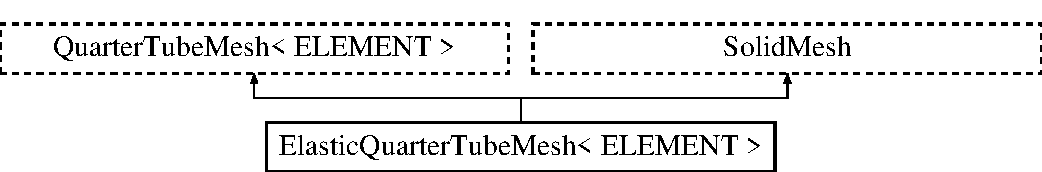
\includegraphics[height=2.000000cm]{classElasticQuarterTubeMesh}
\end{center}
\end{figure}
\subsection*{Public Member Functions}
\begin{DoxyCompactItemize}
\item 
\hyperlink{classElasticQuarterTubeMesh_abb82781bc4c1dc04bdfae437baf49830}{Elastic\+Quarter\+Tube\+Mesh} (Geom\+Object $\ast$wall\+\_\+pt, const Vector$<$ double $>$ \&xi\+\_\+lo, const double \&fract\+\_\+mid, const Vector$<$ double $>$ \&xi\+\_\+hi, const unsigned \&nlayer, Time\+Stepper $\ast$time\+\_\+stepper\+\_\+pt=\&Mesh\+::\+Default\+\_\+\+Time\+Stepper)
\begin{DoxyCompactList}\small\item\em Constructor\+: \end{DoxyCompactList}\item 
virtual \hyperlink{classElasticQuarterTubeMesh_a9ad9db1a8cb86650b505c73fe81eb73c}{$\sim$\+Elastic\+Quarter\+Tube\+Mesh} ()
\begin{DoxyCompactList}\small\item\em Empty Destructor. \end{DoxyCompactList}\end{DoxyCompactItemize}


\subsection{Detailed Description}
\subsubsection*{template$<$class E\+L\+E\+M\+E\+NT$>$\newline
class Elastic\+Quarter\+Tube\+Mesh$<$ E\+L\+E\+M\+E\+N\+T $>$}

Simple quarter tube mesh upgraded to become a solid mesh. 

Definition at line 95 of file three\+\_\+d\+\_\+cantilever.\+cc.



\subsection{Constructor \& Destructor Documentation}
\mbox{\Hypertarget{classElasticQuarterTubeMesh_abb82781bc4c1dc04bdfae437baf49830}\label{classElasticQuarterTubeMesh_abb82781bc4c1dc04bdfae437baf49830}} 
\index{Elastic\+Quarter\+Tube\+Mesh@{Elastic\+Quarter\+Tube\+Mesh}!Elastic\+Quarter\+Tube\+Mesh@{Elastic\+Quarter\+Tube\+Mesh}}
\index{Elastic\+Quarter\+Tube\+Mesh@{Elastic\+Quarter\+Tube\+Mesh}!Elastic\+Quarter\+Tube\+Mesh@{Elastic\+Quarter\+Tube\+Mesh}}
\subsubsection{\texorpdfstring{Elastic\+Quarter\+Tube\+Mesh()}{ElasticQuarterTubeMesh()}}
{\footnotesize\ttfamily template$<$class E\+L\+E\+M\+E\+NT$>$ \\
\hyperlink{classElasticQuarterTubeMesh}{Elastic\+Quarter\+Tube\+Mesh}$<$ E\+L\+E\+M\+E\+NT $>$\+::\hyperlink{classElasticQuarterTubeMesh}{Elastic\+Quarter\+Tube\+Mesh} (\begin{DoxyParamCaption}\item[{Geom\+Object $\ast$}]{wall\+\_\+pt,  }\item[{const Vector$<$ double $>$ \&}]{xi\+\_\+lo,  }\item[{const double \&}]{fract\+\_\+mid,  }\item[{const Vector$<$ double $>$ \&}]{xi\+\_\+hi,  }\item[{const unsigned \&}]{nlayer,  }\item[{Time\+Stepper $\ast$}]{time\+\_\+stepper\+\_\+pt = {\ttfamily \&Mesh\+:\+:Default\+\_\+TimeStepper} }\end{DoxyParamCaption})\hspace{0.3cm}{\ttfamily [inline]}}



Constructor\+: 



Definition at line 102 of file three\+\_\+d\+\_\+cantilever.\+cc.

\mbox{\Hypertarget{classElasticQuarterTubeMesh_a9ad9db1a8cb86650b505c73fe81eb73c}\label{classElasticQuarterTubeMesh_a9ad9db1a8cb86650b505c73fe81eb73c}} 
\index{Elastic\+Quarter\+Tube\+Mesh@{Elastic\+Quarter\+Tube\+Mesh}!````~Elastic\+Quarter\+Tube\+Mesh@{$\sim$\+Elastic\+Quarter\+Tube\+Mesh}}
\index{````~Elastic\+Quarter\+Tube\+Mesh@{$\sim$\+Elastic\+Quarter\+Tube\+Mesh}!Elastic\+Quarter\+Tube\+Mesh@{Elastic\+Quarter\+Tube\+Mesh}}
\subsubsection{\texorpdfstring{$\sim$\+Elastic\+Quarter\+Tube\+Mesh()}{~ElasticQuarterTubeMesh()}}
{\footnotesize\ttfamily template$<$class E\+L\+E\+M\+E\+NT$>$ \\
virtual \hyperlink{classElasticQuarterTubeMesh}{Elastic\+Quarter\+Tube\+Mesh}$<$ E\+L\+E\+M\+E\+NT $>$\+::$\sim$\hyperlink{classElasticQuarterTubeMesh}{Elastic\+Quarter\+Tube\+Mesh} (\begin{DoxyParamCaption}{ }\end{DoxyParamCaption})\hspace{0.3cm}{\ttfamily [inline]}, {\ttfamily [virtual]}}



Empty Destructor. 



Definition at line 117 of file three\+\_\+d\+\_\+cantilever.\+cc.



The documentation for this class was generated from the following file\+:\begin{DoxyCompactItemize}
\item 
\hyperlink{three__d__cantilever_8cc}{three\+\_\+d\+\_\+cantilever.\+cc}\end{DoxyCompactItemize}

\hypertarget{classRefineableElasticQuarterTubeMesh}{}\section{Refineable\+Elastic\+Quarter\+Tube\+Mesh$<$ E\+L\+E\+M\+E\+NT $>$ Class Template Reference}
\label{classRefineableElasticQuarterTubeMesh}\index{Refineable\+Elastic\+Quarter\+Tube\+Mesh$<$ E\+L\+E\+M\+E\+N\+T $>$@{Refineable\+Elastic\+Quarter\+Tube\+Mesh$<$ E\+L\+E\+M\+E\+N\+T $>$}}


Simple quarter tube mesh upgraded to become a solid mesh.  


Inheritance diagram for Refineable\+Elastic\+Quarter\+Tube\+Mesh$<$ E\+L\+E\+M\+E\+NT $>$\+:\begin{figure}[H]
\begin{center}
\leavevmode
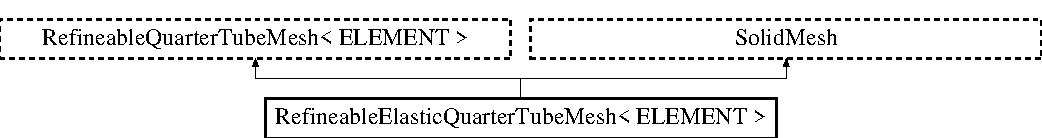
\includegraphics[height=1.854305cm]{classRefineableElasticQuarterTubeMesh}
\end{center}
\end{figure}
\subsection*{Public Member Functions}
\begin{DoxyCompactItemize}
\item 
\hyperlink{classRefineableElasticQuarterTubeMesh_a97c25a8845b2d8ab2a4aef1c0407bacd}{Refineable\+Elastic\+Quarter\+Tube\+Mesh} (Geom\+Object $\ast$wall\+\_\+pt, const Vector$<$ double $>$ \&xi\+\_\+lo, const double \&fract\+\_\+mid, const Vector$<$ double $>$ \&xi\+\_\+hi, const unsigned \&nlayer, Time\+Stepper $\ast$time\+\_\+stepper\+\_\+pt=\&Mesh\+::\+Default\+\_\+\+Time\+Stepper)
\begin{DoxyCompactList}\small\item\em Constructor\+: \end{DoxyCompactList}\item 
virtual \hyperlink{classRefineableElasticQuarterTubeMesh_a157397dff3fb4ab8b1daea787bc9f97c}{$\sim$\+Refineable\+Elastic\+Quarter\+Tube\+Mesh} ()
\begin{DoxyCompactList}\small\item\em Empty Destructor. \end{DoxyCompactList}\end{DoxyCompactItemize}


\subsection{Detailed Description}
\subsubsection*{template$<$class E\+L\+E\+M\+E\+NT$>$\newline
class Refineable\+Elastic\+Quarter\+Tube\+Mesh$<$ E\+L\+E\+M\+E\+N\+T $>$}

Simple quarter tube mesh upgraded to become a solid mesh. 

Definition at line 57 of file three\+\_\+d\+\_\+cantilever.\+cc.



\subsection{Constructor \& Destructor Documentation}
\mbox{\Hypertarget{classRefineableElasticQuarterTubeMesh_a97c25a8845b2d8ab2a4aef1c0407bacd}\label{classRefineableElasticQuarterTubeMesh_a97c25a8845b2d8ab2a4aef1c0407bacd}} 
\index{Refineable\+Elastic\+Quarter\+Tube\+Mesh@{Refineable\+Elastic\+Quarter\+Tube\+Mesh}!Refineable\+Elastic\+Quarter\+Tube\+Mesh@{Refineable\+Elastic\+Quarter\+Tube\+Mesh}}
\index{Refineable\+Elastic\+Quarter\+Tube\+Mesh@{Refineable\+Elastic\+Quarter\+Tube\+Mesh}!Refineable\+Elastic\+Quarter\+Tube\+Mesh@{Refineable\+Elastic\+Quarter\+Tube\+Mesh}}
\subsubsection{\texorpdfstring{Refineable\+Elastic\+Quarter\+Tube\+Mesh()}{RefineableElasticQuarterTubeMesh()}}
{\footnotesize\ttfamily template$<$class E\+L\+E\+M\+E\+NT$>$ \\
\hyperlink{classRefineableElasticQuarterTubeMesh}{Refineable\+Elastic\+Quarter\+Tube\+Mesh}$<$ E\+L\+E\+M\+E\+NT $>$\+::\hyperlink{classRefineableElasticQuarterTubeMesh}{Refineable\+Elastic\+Quarter\+Tube\+Mesh} (\begin{DoxyParamCaption}\item[{Geom\+Object $\ast$}]{wall\+\_\+pt,  }\item[{const Vector$<$ double $>$ \&}]{xi\+\_\+lo,  }\item[{const double \&}]{fract\+\_\+mid,  }\item[{const Vector$<$ double $>$ \&}]{xi\+\_\+hi,  }\item[{const unsigned \&}]{nlayer,  }\item[{Time\+Stepper $\ast$}]{time\+\_\+stepper\+\_\+pt = {\ttfamily \&Mesh\+:\+:Default\+\_\+TimeStepper} }\end{DoxyParamCaption})\hspace{0.3cm}{\ttfamily [inline]}}



Constructor\+: 



Definition at line 65 of file three\+\_\+d\+\_\+cantilever.\+cc.

\mbox{\Hypertarget{classRefineableElasticQuarterTubeMesh_a157397dff3fb4ab8b1daea787bc9f97c}\label{classRefineableElasticQuarterTubeMesh_a157397dff3fb4ab8b1daea787bc9f97c}} 
\index{Refineable\+Elastic\+Quarter\+Tube\+Mesh@{Refineable\+Elastic\+Quarter\+Tube\+Mesh}!````~Refineable\+Elastic\+Quarter\+Tube\+Mesh@{$\sim$\+Refineable\+Elastic\+Quarter\+Tube\+Mesh}}
\index{````~Refineable\+Elastic\+Quarter\+Tube\+Mesh@{$\sim$\+Refineable\+Elastic\+Quarter\+Tube\+Mesh}!Refineable\+Elastic\+Quarter\+Tube\+Mesh@{Refineable\+Elastic\+Quarter\+Tube\+Mesh}}
\subsubsection{\texorpdfstring{$\sim$\+Refineable\+Elastic\+Quarter\+Tube\+Mesh()}{~RefineableElasticQuarterTubeMesh()}}
{\footnotesize\ttfamily template$<$class E\+L\+E\+M\+E\+NT$>$ \\
virtual \hyperlink{classRefineableElasticQuarterTubeMesh}{Refineable\+Elastic\+Quarter\+Tube\+Mesh}$<$ E\+L\+E\+M\+E\+NT $>$\+::$\sim$\hyperlink{classRefineableElasticQuarterTubeMesh}{Refineable\+Elastic\+Quarter\+Tube\+Mesh} (\begin{DoxyParamCaption}{ }\end{DoxyParamCaption})\hspace{0.3cm}{\ttfamily [inline]}, {\ttfamily [virtual]}}



Empty Destructor. 



Definition at line 82 of file three\+\_\+d\+\_\+cantilever.\+cc.



The documentation for this class was generated from the following file\+:\begin{DoxyCompactItemize}
\item 
\hyperlink{three__d__cantilever_8cc}{three\+\_\+d\+\_\+cantilever.\+cc}\end{DoxyCompactItemize}

\chapter{File Documentation}
\hypertarget{three__d__cantilever_8cc}{}\section{three\+\_\+d\+\_\+cantilever.\+cc File Reference}
\label{three__d__cantilever_8cc}\index{three\+\_\+d\+\_\+cantilever.\+cc@{three\+\_\+d\+\_\+cantilever.\+cc}}
\subsection*{Classes}
\begin{DoxyCompactItemize}
\item 
class \hyperlink{classRefineableElasticQuarterTubeMesh}{Refineable\+Elastic\+Quarter\+Tube\+Mesh$<$ E\+L\+E\+M\+E\+N\+T $>$}
\begin{DoxyCompactList}\small\item\em Simple quarter tube mesh upgraded to become a solid mesh. \end{DoxyCompactList}\item 
class \hyperlink{classElasticQuarterTubeMesh}{Elastic\+Quarter\+Tube\+Mesh$<$ E\+L\+E\+M\+E\+N\+T $>$}
\begin{DoxyCompactList}\small\item\em Simple quarter tube mesh upgraded to become a solid mesh. \end{DoxyCompactList}\item 
class \hyperlink{classCantileverProblem}{Cantilever\+Problem$<$ E\+L\+E\+M\+E\+N\+T $>$}
\begin{DoxyCompactList}\small\item\em Problem class for the 3D cantilever \char`\"{}beam\char`\"{} structure. \end{DoxyCompactList}\end{DoxyCompactItemize}
\subsection*{Namespaces}
\begin{DoxyCompactItemize}
\item 
 \hyperlink{namespaceGlobal__Physical__Variables}{Global\+\_\+\+Physical\+\_\+\+Variables}
\begin{DoxyCompactList}\small\item\em Global variables. \end{DoxyCompactList}\end{DoxyCompactItemize}
\subsection*{Functions}
\begin{DoxyCompactItemize}
\item 
void \hyperlink{namespaceGlobal__Physical__Variables_a0777aef63372db7f91ad894c38159681}{Global\+\_\+\+Physical\+\_\+\+Variables\+::gravity} (const double \&time, const Vector$<$ double $>$ \&xi, Vector$<$ double $>$ \&b)
\begin{DoxyCompactList}\small\item\em Non-\/dimensional gravity as body force. \end{DoxyCompactList}\item 
int \hyperlink{three__d__cantilever_8cc_a0ddf1224851353fc92bfbff6f499fa97}{main} (int argc, char $\ast$argv\mbox{[}$\,$\mbox{]})
\begin{DoxyCompactList}\small\item\em Driver for 3D cantilever beam loaded by gravity. \end{DoxyCompactList}\end{DoxyCompactItemize}
\subsection*{Variables}
\begin{DoxyCompactItemize}
\item 
double \hyperlink{namespaceGlobal__Physical__Variables_a1b8bfc451f6b7ac89eca18f04338f47f}{Global\+\_\+\+Physical\+\_\+\+Variables\+::L} =10.\+0
\begin{DoxyCompactList}\small\item\em Length of beam. \end{DoxyCompactList}\item 
Strain\+Energy\+Function $\ast$ \hyperlink{namespaceGlobal__Physical__Variables_a73135f793690b4386bf83bbefc7bf310}{Global\+\_\+\+Physical\+\_\+\+Variables\+::\+Strain\+\_\+energy\+\_\+function\+\_\+pt} =0
\begin{DoxyCompactList}\small\item\em Pointer to strain energy function. \end{DoxyCompactList}\item 
double \hyperlink{namespaceGlobal__Physical__Variables_a849754fa7155c1a31481674ce4845658}{Global\+\_\+\+Physical\+\_\+\+Variables\+::\+C1} =1.\+3
\begin{DoxyCompactList}\small\item\em First \char`\"{}\+Mooney Rivlin\char`\"{} coefficient. \end{DoxyCompactList}\item 
double \hyperlink{namespaceGlobal__Physical__Variables_af9defd1b5745cce50d2c386b3ac0e0ae}{Global\+\_\+\+Physical\+\_\+\+Variables\+::\+C2} =1.\+3
\begin{DoxyCompactList}\small\item\em Second \char`\"{}\+Mooney Rivlin\char`\"{} coefficient. \end{DoxyCompactList}\item 
Constitutive\+Law $\ast$ \hyperlink{namespaceGlobal__Physical__Variables_a2a37fb040c832ee7a086bb13bb02a100}{Global\+\_\+\+Physical\+\_\+\+Variables\+::\+Constitutive\+\_\+law\+\_\+pt} =0
\begin{DoxyCompactList}\small\item\em Pointer to constitutive law. \end{DoxyCompactList}\item 
double \hyperlink{namespaceGlobal__Physical__Variables_a8b80d3e8d63b8d0a0ed435a2dd7fe2ad}{Global\+\_\+\+Physical\+\_\+\+Variables\+::\+Gravity} =0.\+0
\begin{DoxyCompactList}\small\item\em Non-\/dim gravity. \end{DoxyCompactList}\item 
double \hyperlink{namespaceGlobal__Physical__Variables_a09a019474b7405b35da2437f7779bc7e}{Global\+\_\+\+Physical\+\_\+\+Variables\+::E} =1.\+0
\begin{DoxyCompactList}\small\item\em Elastic modulus. \end{DoxyCompactList}\item 
double \hyperlink{namespaceGlobal__Physical__Variables_a3962c36313826b19f216f6bbbdd6a477}{Global\+\_\+\+Physical\+\_\+\+Variables\+::\+Nu} =0.\+3
\begin{DoxyCompactList}\small\item\em Poisson\textquotesingle{}s ratio. \end{DoxyCompactList}\end{DoxyCompactItemize}


\subsection{Function Documentation}
\mbox{\Hypertarget{three__d__cantilever_8cc_a0ddf1224851353fc92bfbff6f499fa97}\label{three__d__cantilever_8cc_a0ddf1224851353fc92bfbff6f499fa97}} 
\index{three\+\_\+d\+\_\+cantilever.\+cc@{three\+\_\+d\+\_\+cantilever.\+cc}!main@{main}}
\index{main@{main}!three\+\_\+d\+\_\+cantilever.\+cc@{three\+\_\+d\+\_\+cantilever.\+cc}}
\subsubsection{\texorpdfstring{main()}{main()}}
{\footnotesize\ttfamily int main (\begin{DoxyParamCaption}\item[{int}]{argc,  }\item[{char $\ast$}]{argv\mbox{[}$\,$\mbox{]} }\end{DoxyParamCaption})}



Driver for 3D cantilever beam loaded by gravity. 



Definition at line 477 of file three\+\_\+d\+\_\+cantilever.\+cc.



References Global\+\_\+\+Physical\+\_\+\+Variables\+::\+C1, Global\+\_\+\+Physical\+\_\+\+Variables\+::\+C2, Global\+\_\+\+Physical\+\_\+\+Variables\+::\+Constitutive\+\_\+law\+\_\+pt, Cantilever\+Problem$<$ E\+L\+E\+M\+E\+N\+T $>$\+::doc\+\_\+solution(), Global\+\_\+\+Physical\+\_\+\+Variables\+::E, Global\+\_\+\+Physical\+\_\+\+Variables\+::\+Gravity, Global\+\_\+\+Physical\+\_\+\+Variables\+::\+Nu, Cantilever\+Problem$<$ E\+L\+E\+M\+E\+N\+T $>$\+::run\+\_\+tests(), and Global\+\_\+\+Physical\+\_\+\+Variables\+::\+Strain\+\_\+energy\+\_\+function\+\_\+pt.


\hypertarget{three__d__cantilever_8txt__doxygenified_8h}{}\section{three\+\_\+d\+\_\+cantilever.\+txt\+\_\+doxygenified.\+h File Reference}
\label{three__d__cantilever_8txt__doxygenified_8h}\index{three\+\_\+d\+\_\+cantilever.\+txt\+\_\+doxygenified.\+h@{three\+\_\+d\+\_\+cantilever.\+txt\+\_\+doxygenified.\+h}}

%--- End generated contents ---

% Index
\backmatter
\newpage
\phantomsection
\clearemptydoublepage
\addcontentsline{toc}{chapter}{Index}
\printindex

\end{document}
